% === T01 - Introducción a FPGAs ===
% David Alejandro Gonzalez Marquez
% fokerman@gmail.com
% https://github.com/fokerman/fpgaSoftcoreProgrammingCourse

\RequirePackage[2020-02-02]{latexrelease}

\documentclass[aspectratio=169]{beamer}
\usepackage{../packages}
% handout
\newcommand{\na}{\cellcolor{naranjauca}}
\newcommand{\gm}{\cellcolor{gray!50}}

\title{\Huge Introducción a FPGAs\\ \large y repaso de Lógica Digital}
\author{David Alejandro González Márquez}
\institute{Programación de softcores en FPGAs\\
Programa de Profesoras/es Visitantes\\
Departamento de computación\\
Universidad de Buenos Aires}


\date{}

\begin{document}

\begin{frame}[plain]
    \titlepage
    \begin{textblock}{110}(25,80)
    \begin{tcolorbox}[size=small,width=\textwidth,colback={gray!30},title={}]
    \begin{center}
     \scriptsize Clase disponible en: \url{https://github.com/fokerman/fpgaSoftcoreProgrammingCourse}
    \end{center}
    \end{tcolorbox}
    \end{textblock}
\end{frame}

\begin{frame}[fragile]
    \frametitle{\large La materia: \Large Programación de Softcores en FPGAs}
    \textbf{Objetivo de este curso:}\\
    \vspace{-0.4cm}
    \begin{center}
    \textcolor{verdeuca}{El aprendizaje de la programación de FPGAs guiada por el desarrollo de \emph{softcores processors}.}\\
    \end{center}
    \pause
    \textbf{Temas y calendario:}\\
    \vspace{-0.2cm}
    \begin{itemize}
    \setlength\itemsep{0.0cm}
     \item[T0] Repaso de \textcolor{naranjauca}{lógica digital} e Introducción a las FPGAs
     \item[T1] Lenguajes de descripción de Hardware, \textcolor{naranjauca}{Verilog}.
     \item[T2] Modelo de \textcolor{naranjauca}{tiempos} y delay. Definición de \textcolor{naranjauca}{Testbench}.
     \pause
     \item[T3] \textcolor{naranjauca}{Arquitectura} de procesadores, modelos de cómputo.
     \item[T4] \textcolor{naranjauca}{Microarquitectura}, diseños de múltiples ciclos y un solo ciclo.
     \item[T5] Técnicas de segmentación de instrucciones (\textcolor{naranjauca}{pipeline}). Diseño de etapas y tiempos.
     \pause
     \item[T6] Introducción a \textcolor{naranjauca}{softcores}: Picoblaze y Microblaze, características y casos de uso. Modelado e interacción entre múltiples cores.
    \end{itemize}
    \pause
    \textbf{Clases:}\\
    \vspace{-0.2cm}
    \begin{itemize}
    \item \textcolor{verdeuca}{
    Todas las clases van a estar disponibles en \texttt{github} con sus fuentes.\\
    Son libres de enviar PRs para mejorar el material o incluso agregar comentarios.\\}
    \end{itemize}
\end{frame}

\begin{frame}[fragile]
    \frametitle{\large La materia: \Large Programación de Softcores en FPGAs}
    \textbf{Requerimientos:}
    \begin{itemize}
    \item Notebook con Linux + Software de diseño \texttt{Vivado} de \texttt{Xilinx}.\\
    \end{itemize}
    \pause
    \vspace{0.2cm}
    \textbf{Material de estudio y práctica:}
    \begin{itemize}
    \item Clases teóricas y prácticas.
    \item Guía práctica de ejercicios de Verilog.
    \item Bibliografía y Papers.
    \end{itemize}
    \pause
    \vspace{0.2cm}
    \textbf{Forma de evaluación:}
    \begin{itemize}
    \item Trabajo Práctico de Microarquitectura $\rightarrow$ \textcolor{verdeuca}{Nota númerica grupal.}\\
    \item Presentación de temas $\rightarrow$ \textcolor{verdeuca}{Presentación en clase en grupo.}\\
    \item Evaluación oral/escrita de final de curso $\rightarrow$ \textcolor{verdeuca}{Nota númerica.}\\
    \end{itemize}
    \pause
    \vspace{0.2cm}
    \textbf{Calificación final:}
    \begin{itemize}
     \item Promedio entre evaluación final y trabajo práctico.\\
    \end{itemize}
\end{frame}

\begin{frame}[fragile]
    \frametitle{Bibliografía}
    \begin{itemize}
    \setlength\itemsep{0.1cm}
    \footnotesize
    \item[-] \textbf{``Digital Design and Computer Architecture''}, Second Edition\\
    David Money Harris, Sarah L. Harris - Morgan Kaufmann - 2013\\    
    \item[-] \textbf{``Diseño Digital''}, Tercera Edición\\
    M. Morris Mano - Pearson - 2003\\
    \item[-] \textbf{“Essentials of Computer Organization and Architecture”}, 5th Edition\\
    Linda Null, Julia Lobur - Jones and Bartlett Publishers - 2018.\\
    \item[-] \textbf{``Introduction to Computing Systems''}, Third Edition\\
    Yale N. Patt, Sanjay J. Patel - McGraw-Hill - 2019\\
    \item[-] \textbf{``Computer Organization and Design: The Hardware/Software Interface''}, Fifth Edition\\
    David A. Patterson, John L. Hennessy - Morgan Kaufmann - 2014\\
    \item[-] \textbf{``Syntesis of Arithmetic Circuits FPGA, ASIC, and Embedded Systems''}\\
    Jean-Pierre Deschamps, Gery Jean Antoine Biol, Gustavo D. Sutter - John Wiley \& Sons - 2006\\
    \item[-] \textbf{``CMOS VLSI Design: A Circuits and Systems Perspective''}, Fourth Edition.\\
    Neil H. E. Weste, David Money Harris - Pearson - 2011\\
    \item[-] \textbf{``Computer Architecture: A Quantitative Approach''}, Sixth Edition.\\
    John L. Hennessy, David A. Patterson - Morgan Kaufmann - 2019\\
    \item[-] \textbf{``Digital Design and Verilog HDL Fundamentals''}\\
    Joseph Cavanagh - CRC Press, Taylor \& Francis Group - 2008\\
    \end{itemize}
\end{frame}

\begin{frame}[fragile]
    \frametitle{Agenda}
    \Large
    \begin{enumerate}
    \setlength\itemsep{1cm}
    \item[\LARGE 1 - ] Repaso de Lógica Digital
    \item[\LARGE 2 - ] Introducción a los FPGAs
    \end{enumerate}
\end{frame}

\begin{frame}[fragile,t]
    \frametitle{Componentes Básicos: Compuertas}
    Las compuertas nos permiten hacer operaciones con las señales eléctricas (\texttt{0} y \texttt{1}).\\
    \bigskip
    Vamos a utilizar compuertas para construir circuitos que respeten el comportamiento de una determinada función.
    Estos circuitos se denominan \textbf{combinatorios}.
    \bigskip
    \begin{textblock}{16}(8,37)   \begin{center} \includegraphics[scale=0.6]{img/compuertas-layer1.pdf} \end{center} \end{textblock}
    \begin{textblock}{21}(28,37)  \begin{center} \includegraphics[scale=0.6]{img/compuertas-layer2.pdf} \end{center} \end{textblock}
    \begin{textblock}{21}(53,37)  \begin{center} \includegraphics[scale=0.6]{img/compuertas-layer3.pdf} \end{center} \end{textblock}
    \begin{textblock}{21}(77,37)  \begin{center} \includegraphics[scale=0.6]{img/compuertas-layer4.pdf} \end{center} \end{textblock}
    \begin{textblock}{21}(105,37) \begin{center} \includegraphics[scale=0.6]{img/compuertas-layer5.pdf} \end{center} \end{textblock}
    \begin{textblock}{21}(130,37) \begin{center} \includegraphics[scale=0.6]{img/compuertas-layer6.pdf} \end{center} \end{textblock}
    \begin{textblock}{100}(8,50)
    \begin{tabular}{c|c}
    \multicolumn{2}{c}{\textcolor{naranjauca}{ $\overline{\texttt{A}}$ } } \\
    \texttt{A} & \texttt{NOT} \\
    \hline
    \texttt{0} & \texttt{1} \\
    \texttt{1} & \texttt{0} \\
    \end{tabular}
    \end{textblock}
    \begin{textblock}{100}(28,50)
    \begin{tabular}{cc|c}
    \multicolumn{3}{c}{\textcolor{naranjauca}{ $\texttt{A}\cdot\texttt{B}$ } } \\
    \texttt{A} & \texttt{B} & \texttt{AND} \\
    \hline
    \texttt{0} & \texttt{0} & \texttt{0} \\
    \texttt{0} & \texttt{1} & \texttt{0} \\
    \texttt{1} & \texttt{0} & \texttt{0} \\
    \texttt{1} & \texttt{1} & \texttt{1} \\
    \end{tabular}
    \end{textblock}
    \begin{textblock}{100}(53,50)
    \begin{tabular}{cc|c}
    \multicolumn{3}{c}{\textcolor{naranjauca}{ $\texttt{A}+\texttt{B}$ } } \\
    \texttt{A} & \texttt{B} & \texttt{OR} \\
    \hline
    \texttt{0} & \texttt{0} & \texttt{0} \\
    \texttt{0} & \texttt{1} & \texttt{1} \\
    \texttt{1} & \texttt{0} & \texttt{1} \\
    \texttt{1} & \texttt{1} & \texttt{1} \\
    \end{tabular}
    \end{textblock}
    \begin{textblock}{100}(77,50)
    \begin{tabular}{cc|c}
    \multicolumn{3}{c}{\textcolor{naranjauca}{ $\overline{\texttt{A}\cdot\texttt{B}}$ } } \\
    \texttt{A} & \texttt{B} & \texttt{NAND} \\
    \hline
    \texttt{0} & \texttt{0} & \texttt{1} \\
    \texttt{0} & \texttt{1} & \texttt{1} \\
    \texttt{1} & \texttt{0} & \texttt{1} \\
    \texttt{1} & \texttt{1} & \texttt{0} \\
    \end{tabular}
    \end{textblock}
    \begin{textblock}{100}(105,50)
    \begin{tabular}{cc|c}
    \multicolumn{3}{c}{\textcolor{naranjauca}{ $\overline{\texttt{A}+\texttt{B}}$ } } \\
    \texttt{A} & \texttt{B} & \texttt{NOR} \\
    \hline
    \texttt{0} & \texttt{0} & \texttt{1} \\
    \texttt{0} & \texttt{1} & \texttt{0} \\
    \texttt{1} & \texttt{0} & \texttt{0} \\
    \texttt{1} & \texttt{1} & \texttt{0} \\
    \end{tabular}
    \end{textblock}
    \begin{textblock}{100}(130,50)
    \begin{tabular}{cc|c}
    \multicolumn{3}{c}{\textcolor{naranjauca}{ $\texttt{A}\oplus\texttt{B}$ } } \\
    \texttt{A} & \texttt{B} & \texttt{XOR} \\
    \hline
    \texttt{0} & \texttt{0} & \texttt{0} \\
    \texttt{0} & \texttt{1} & \texttt{1} \\
    \texttt{1} & \texttt{0} & \texttt{1} \\
    \texttt{1} & \texttt{1} & \texttt{0} \\
    \end{tabular}
    \end{textblock}
\end{frame}

\begin{frame}[fragile,t]
    \frametitle{Construir funciones booleanas con su tabla de verdad}
    Dos formas canónicas de expresiones booleanas:
    \pause
    \begin{itemize}
    \item \textcolor{naranjauca}{Suma de Productos}\\
    \small Expresión que hace la suma de todas las combinaciones que resulten en 1.
    \pause
    \item \textcolor{naranjauca}{Producto de Sumas}\\
    \small Expresión que hace el producto de todas las combinaciones que resulten en 0.
    \pause
    \end{itemize}
    \bigskip
    \textcolor{gray}{Ejemplo:}\\
    \bigskip
    \begin{tabular}{|c|c|c|}
    \hline
    $A$ & $B$ & $F(A,B)$ \\
    \hline
    $0$ & $0$ & \textcolor{azul}{$1$} \\
    $0$ & $1$ & \textcolor{verde}{$0$} \\
    $1$ & $0$ & \textcolor{rojo}{$1$} \\
    $1$ & $1$ & \textcolor{amarillo}{$0$} \\
    \hline
    \end{tabular}
    \begin{textblock}{100}(50,50)
    \uncover<4->{ \small \textcolor{naranjauca}{Suma de Productos}\\
    \large
    $F(A,B)$ = $ \textcolor{azul}{( \overline{A} \cdot \overline{B} )} + \textcolor{rojo}{( A \cdot \overline{B} )} $\\ }
    \bigskip    
    \uncover<5->{ \small \textcolor{naranjauca}{Producto de Sumas}\\
    \large
    $F(A,B)$ = $ \textcolor{verde}{( A + \overline{B} )} \cdot \textcolor{amarillo}{( \overline{A} + \overline{B} )} $  }
    \end{textblock}
\end{frame}

\begin{frame}[fragile,t]
    \frametitle{Construir circuitos a partir de una función booleana}
    \textcolor{gray}{Ejemplo:}\\
    \bigskip
    \begin{tabular}{|c|c|c|}
    \hline
    $A$ & $B$ & $F(A,B)$ \\
    \hline
    $0$ & $0$ & \textcolor{azul}{$1$} \\
    $0$ & $1$ & \textcolor{verde}{$0$} \\
    $1$ & $0$ & \textcolor{rojo}{$1$} \\
    $1$ & $1$ & \textcolor{amarillo}{$0$} \\
    \hline
    \end{tabular}
    \begin{textblock}{100}(10,50)
    \small \textcolor{naranjauca}{Suma de Productos}\\
    \large
    $F(A,B)$ = $ \textcolor{azul}{( \overline{A} \cdot \overline{B} )} + \textcolor{rojo}{( A \cdot \overline{B} )} $\\
    \bigskip
    \small \textcolor{naranjauca}{Producto de Sumas}\\
    \large
    $F(A,B)$ = $ \textcolor{verde}{( A + \overline{B} )} \cdot \textcolor{amarillo}{( \overline{A} + \overline{B} )} $ 
    \end{textblock}
    \begin{textblock}{100}(100,16) \only<2->{\small \textcolor{naranjauca}{Suma de Productos}} \end{textblock}
    \begin{textblock}{100}(80,15)  \only<3->{\includegraphics[scale=0.8]{img/circuitoEjemploFAB1010-layer1.pdf}} \end{textblock}
    \begin{textblock}{100}(80,15)  \only<3->{\includegraphics[scale=0.8]{img/circuitoEjemploFAB1010-layer2.pdf}} \end{textblock}
    \begin{textblock}{100}(80,15)  \only<3->{\includegraphics[scale=0.8]{img/circuitoEjemploFAB1010-layer3.pdf}} \end{textblock}
    \begin{textblock}{100}(80,15)  \only<3->{\includegraphics[scale=0.8]{img/circuitoEjemploFAB1010-layer4.pdf}} \end{textblock}
    \begin{textblock}{100}(80,15)  \only<3->{\includegraphics[scale=0.8]{img/circuitoEjemploFAB1010-layer5.pdf}} \end{textblock}
    \begin{textblock}{100}(100,51) \only<4->{\small \textcolor{naranjauca}{Producto de Sumas}} \end{textblock}
    \begin{textblock}{100}(80,50)  \only<5->{\includegraphics[scale=0.8]{img/circuitoEjemploFAB1010-layer6.pdf}} \end{textblock}
    \begin{textblock}{100}(80,50)  \only<5->{\includegraphics[scale=0.8]{img/circuitoEjemploFAB1010-layer7.pdf}} \end{textblock}
    \begin{textblock}{100}(80,50)  \only<5->{\includegraphics[scale=0.8]{img/circuitoEjemploFAB1010-layer8.pdf}} \end{textblock}
    \begin{textblock}{100}(80,50)  \only<5->{\includegraphics[scale=0.8]{img/circuitoEjemploFAB1010-layer9.pdf}} \end{textblock}
    \begin{textblock}{100}(80,50)  \only<5->{\includegraphics[scale=0.8]{img/circuitoEjemploFAB1010-layer10.pdf}} \end{textblock}
\end{frame}

\begin{frame}[fragile,t]
    \frametitle{Construir circuitos a partir de una función booleana}
    \textcolor{gray}{Ejemplo:}\\
    \bigskip
    \begin{tabular}{|c|c|c|}
    \hline
    $A$ & $B$ & $F(A,B)$ \\
    \hline
    $0$ & $0$ & \textcolor{azul}{$1$} \\
    $0$ & $1$ & \textcolor{verde}{$0$} \\
    $1$ & $0$ & \textcolor{rojo}{$1$} \\
    $1$ & $1$ & \textcolor{amarillo}{$0$} \\
    \hline
    \end{tabular}
    \begin{textblock}{100}(10,50)
    \small \textcolor{naranjauca}{Suma de Productos}\\
    \large
    $F(A,B)$ = $ \textcolor{azul}{( \overline{A} \cdot \overline{B} )} + \textcolor{rojo}{( A \cdot \overline{B} )} $\\
    \bigskip
    \small \textcolor{naranjauca}{Producto de Sumas}\\
    \large
    $F(A,B)$ = $ \textcolor{verde}{( A + \overline{B} )} \cdot \textcolor{amarillo}{( \overline{A} + \overline{B} )} $ 
    \end{textblock}
    \begin{textblock}{100}(60,15)
    \only<2->{
    \small \textcolor{naranjauca}{Suma de Productos}\\
    $F(A,B)$ = $( \overline{A} \cdot \overline{B} ) + ( A \cdot \overline{B} )$\\
    $F(A,B)$ = $( \overline{A} +  A ) \cdot \overline{B} $\\
    $F(A,B)$ = $1 \cdot \overline{B} $\\
    $F(A,B)$ = $\overline{B}$
    }
    \end{textblock}
    \begin{textblock}{100}(110,15)
    \only<3->{
    \small \textcolor{naranjauca}{Producto de Sumas}\\
    $F(A,B)$ = $( A + \overline{B} ) \cdot ( \overline{A} + \overline{B} )$\\
    $F(A,B)$ = $( A \cdot \overline{A} ) + \overline{B}$\\
    $F(A,B)$ = $ 0 + \overline{B}$\\
    $F(A,B)$ = $ \overline{B}$
    }
    \end{textblock}
    \begin{textblock}{100}(100,51) \only<4->{\small \textcolor{naranjauca}{Expresión reducida}} \end{textblock}
    \begin{textblock}{100}(80,50)  \only<4->{\includegraphics[scale=0.8]{img/circuitoEjemploFAB1010-layer11.pdf}} \end{textblock}
    \begin{textblock}{100}(80,50)  \only<4->{\includegraphics[scale=0.8]{img/circuitoEjemploFAB1010-layer12.pdf}} \end{textblock}
\end{frame}

\begin{frame}[fragile]
    \frametitle{Uso de compuertas para seleccionar y habilitar}
    \begin{textblock}{100}(10,25)   \only<1->{\textcolor{naranjauca}{Habilitar}} \end{textblock}
    \begin{textblock}{100}(30,15)   \only<1->{\includegraphics[scale=1]{img/propiedadesCompuertas-layer1.pdf}} \end{textblock}
    \begin{textblock}{100}(30,30)   \only<1->{\includegraphics[scale=1]{img/propiedadesCompuertas-layer2.pdf}} \end{textblock}
    \begin{textblock}{100}(55,17.5) \only<1->{\texttt{AND} de \texttt{X} y \texttt{1} deja pasar \texttt{X}} \end{textblock}
    \begin{textblock}{100}(55,32.5) \only<1->{\texttt{AND} de \texttt{X} y \texttt{0} no deja pasar \texttt{X}} \end{textblock}
    \begin{textblock}{100}(10,60)   \only<2->{\textcolor{naranjauca}{Seleccionar}} \end{textblock}
    \begin{textblock}{100}(30,50)   \only<2->{\includegraphics[scale=1]{img/propiedadesCompuertas-layer3.pdf}} \end{textblock}
    \begin{textblock}{100}(30,65)   \only<2->{\includegraphics[scale=1]{img/propiedadesCompuertas-layer4.pdf}} \end{textblock}
    \begin{textblock}{100}(55,52.5) \only<2->{\texttt{OR} de \texttt{X} y \texttt{0} deja pasar \texttt{X}} \end{textblock}
    \begin{textblock}{100}(55,67.5) \only<2->{\texttt{OR} de \texttt{Y} y \texttt{0} deja pasar \texttt{Y}} \end{textblock}
    \begin{textblock}{50}(105,10) \only<3->{
        \begin{block}{\small Ejemplo}
        \begin{center}
        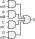
\includegraphics[scale=0.8]{img/enable4bits.pdf}
        \end{center}
        \small
        Las señales \texttt{enA}, \texttt{enB}, \texttt{enC} y \texttt{enD} son de habilitación, para los datos de las señales \texttt{A}, \texttt{B}, \texttt{C} y \texttt{D}.
        \end{block}
    }
    \end{textblock}
\end{frame}

\begin{frame}[fragile]
    \frametitle{Circuitos Combinatorios: Decodificadores y Codificadores}
    \begin{textblock}{100}(10,15) Decodificador \end{textblock}
    \begin{textblock}{100}(10,23) \includegraphics[scale=0.9]{img/cirMuxDemuxCodeDecode-layer4.pdf} \end{textblock}
    \begin{textblock}{100}(50,15)
    \small Circuito que toma $n$ entradas ($\mathrm{e_0}$ a $\mathrm{e_{n-1}}$) y genera $\mathrm{2^n}$ salidas ($\mathrm{s_0}$ a $\mathrm{s_{2^n-1}}$).\\
    \bigskip
    Coloca un \texttt{1} en la salida codificada por la entrada.\\ El resto de las salidas quedan en \texttt{0}.
    \end{textblock}
    \begin{textblock}{100}(10,50)  \only<2->{ \textcolor{gray}{Ejemplo} - \small Decodificador de 2 entradas } \end{textblock}
    \begin{textblock}{100}(3, 60)  \only<2->{ \includegraphics[scale=0.8]{img/exDecoCode-layer1.pdf} } \end{textblock}
    \begin{textblock}{100}(43,60)  \only<2->{ \includegraphics[scale=0.8]{img/exDecoCode-layer2.pdf} } \end{textblock}
    \begin{textblock}{100}(83,60)  \only<2->{ \includegraphics[scale=0.8]{img/exDecoCode-layer3.pdf} } \end{textblock}
    \begin{textblock}{100}(123,60) \only<2->{ \includegraphics[scale=0.8]{img/exDecoCode-layer4.pdf} } \end{textblock}
\end{frame}

\begin{frame}[fragile]
    \frametitle{Circuitos Combinatorios: Decodificadores y Codificadores}
    \begin{textblock}{100}(10,15) Codificador \end{textblock}
    \begin{textblock}{100}(10,23) \includegraphics[scale=0.9]{img/cirMuxDemuxCodeDecode-layer3.pdf} \end{textblock}
    \begin{textblock}{100}(50,15)
    \small Circuito que toma $\mathrm{2^n}$ entradas ($\mathrm{e_0}$ a $\mathrm{e_{2^n-1}}$) y genera $n$ salidas ($\mathrm{s_0}$ a $\mathrm{s_{n-1}}$).\\
    \bigskip
    Expone en las salidas la codificación de la única entrada en \texttt{1}.\\ Este circuito no permite que más de una entrada esté en \texttt{1}. 
    \end{textblock}
    \begin{textblock}{100}(10,50)  \only<2->{ \textcolor{gray}{Ejemplo} - \small Codificador de 4 entradas } \end{textblock}
    \begin{textblock}{100}(4,60)  \only<2->{ \includegraphics[scale=0.8]{img/exDecoCode-layer5.pdf} } \end{textblock}
    \begin{textblock}{100}(44,60)  \only<2->{ \includegraphics[scale=0.8]{img/exDecoCode-layer6.pdf} } \end{textblock}
    \begin{textblock}{100}(84,60)  \only<2->{ \includegraphics[scale=0.8]{img/exDecoCode-layer7.pdf} } \end{textblock}
    \begin{textblock}{100}(124,60) \only<2->{ \includegraphics[scale=0.8]{img/exDecoCode-layer8.pdf} } \end{textblock}
\end{frame}

\begin{frame}[fragile]
    \frametitle{Circuitos Combinatorios: Decodificadores y Codificadores}
    \begin{textblock}{100}(10,15) \only<1->{ Decodificador } \end{textblock}
    \begin{textblock}{100}(10,23) \only<1->{ \includegraphics[scale=0.9]{img/cirMuxDemuxCodeDecode-layer4.pdf} } \end{textblock}
    \begin{textblock}{100}(51,15) \only<2->{
    \begin{tabular}{|cc|cccc|}  \hline
    \multicolumn{2}{|c|}{\small entradas} & \multicolumn{4}{c|}{\small salida} \\  \hline
    \small\texttt{E$_1$} & \small\texttt{E$_0$} & \small\texttt{S$_0$} & \small\texttt{S$_1$} & \small\texttt{S$_2$} & \small\texttt{S$_3$} \\ \hline
    \small\texttt{0}     & \small\texttt{0}     & \small\texttt{1}     & \small\texttt{0}     & \small\texttt{0}     & \small\texttt{0}     \\
    \small\texttt{0}     & \small\texttt{1}     & \small\texttt{0}     & \small\texttt{1}     & \small\texttt{0}     & \small\texttt{0}     \\
    \small\texttt{1}     & \small\texttt{0}     & \small\texttt{0}     & \small\texttt{0}     & \small\texttt{1}     & \small\texttt{0}     \\
    \small\texttt{1}     & \small\texttt{1}     & \small\texttt{0}     & \small\texttt{0}     & \small\texttt{0}     & \small\texttt{1}     \\ \hline
    \end{tabular} }
    \end{textblock}
    \begin{textblock}{100}(112,15)  \only<3->{ 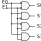
\includegraphics[scale=0.5]{img/decode.pdf} } \end{textblock}
    \begin{textblock}{100}(10,52) \only<1->{ Codificador } \end{textblock}
    \begin{textblock}{100}(10,60) \only<1->{ \includegraphics[scale=0.9]{img/cirMuxDemuxCodeDecode-layer3.pdf} } \end{textblock}
    \begin{textblock}{100}(52,52) \only<4->{
    \begin{tabular}{|cccc|cc|}  \hline
    \multicolumn{4}{|c|}{\small entradas} & \multicolumn{2}{c|}{\small salidas} \\  \hline
    \small\texttt{E$_0$} & \small\texttt{E$_1$} & \small\texttt{E$_2$} & \small\texttt{E$_3$} & \small\texttt{S$_1$} & \small\texttt{S$_0$} \\ \hline
    \small\texttt{1}     & \small\texttt{0}     & \small\texttt{0}     & \small\texttt{0}     & \small\texttt{0}     & \small\texttt{0} \\
    \small\texttt{0}     & \small\texttt{1}     & \small\texttt{0}     & \small\texttt{0}     & \small\texttt{0}     & \small\texttt{1} \\
    \small\texttt{0}     & \small\texttt{0}     & \small\texttt{1}     & \small\texttt{0}     & \small\texttt{1}     & \small\texttt{0} \\
    \small\texttt{0}     & \small\texttt{0}     & \small\texttt{0}     & \small\texttt{1}     & \small\texttt{1}     & \small\texttt{1} \\ \hline
    \end{tabular} }
    \end{textblock}
    \begin{textblock}{100}(112,52)  \only<5->{ 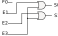
\includegraphics[scale=0.5]{img/encode.pdf} } \end{textblock}
\end{frame}

\begin{frame}[fragile]
    \frametitle{Circuitos Combinatorios: Multiplexores y Demultiplexores}
    \begin{textblock}{100}(10,15) Multiplexor \end{textblock}
    \begin{textblock}{100}(10,23) \includegraphics[scale=0.9]{img/cirMuxDemuxCodeDecode-layer1.pdf} \end{textblock}
    \begin{textblock}{100}(50,15)
    \small Circuito que toma $n$ entradas de control ($\mathrm{c_0}$ a $\mathrm{c_{n-1}}$), $\mathrm{2^n}$ entradas de datos ($\mathrm{e_0}$ a $\mathrm{e_{2^n-1}}$) y genera una salida $s_0$.\\
    \bigskip
    Dependiendo del valor de las entradas de control, selecciona una de las entradas de datos y la expone en la salida.
    \end{textblock}
    \begin{textblock}{100}(10,50)  \only<2->{ \textcolor{gray}{Ejemplo} - \small Multiplexor de 4 entradas } \end{textblock}
    \begin{textblock}{100}(10,60)  \only<2->{ \includegraphics[scale=0.8]{img/exMuxDemux-layer1.pdf} } \end{textblock}
    \begin{textblock}{100}(45,60)  \only<2->{ \includegraphics[scale=0.8]{img/exMuxDemux-layer2.pdf} } \end{textblock}
    \begin{textblock}{100}(80,60)  \only<2->{ \includegraphics[scale=0.8]{img/exMuxDemux-layer3.pdf} } \end{textblock}
    \begin{textblock}{100}(115,60) \only<2->{ \includegraphics[scale=0.8]{img/exMuxDemux-layer4.pdf} } \end{textblock}
\end{frame}

\begin{frame}[fragile]
    \frametitle{Circuitos Combinatorios: Multiplexores y Demultiplexores}
    \begin{textblock}{100}(10,15) Demultiplexor \end{textblock}
    \begin{textblock}{100}(10,23) \includegraphics[scale=0.9]{img/cirMuxDemuxCodeDecode-layer2.pdf} \end{textblock}
    \begin{textblock}{100}(50,15)
    \small Circuito que toma $n$ entradas de control ($\mathrm{c_0}$ a $\mathrm{c_{n-1}}$), una entrada de datos $\mathrm{e_0}$ y genera $\mathrm{2^n}$ salidas ($\mathrm{s_0}$ a $\mathrm{s_{2^n-1}}$).\\
    \bigskip
    Expone la entrada en una de las salidas, dependiendo del valor de las entradas de control.
    \end{textblock}
    \begin{textblock}{100}(10,50)  \only<2->{ \textcolor{gray}{Ejemplo} - \small Demultiplexor de 4 entradas } \end{textblock}
    \begin{textblock}{100}(10,60)  \only<2->{ \includegraphics[scale=0.8]{img/exMuxDemux-layer5.pdf} } \end{textblock}
    \begin{textblock}{100}(45,60)  \only<2->{ \includegraphics[scale=0.8]{img/exMuxDemux-layer6.pdf} } \end{textblock}
    \begin{textblock}{100}(80,60)  \only<2->{ \includegraphics[scale=0.8]{img/exMuxDemux-layer7.pdf} } \end{textblock}
    \begin{textblock}{100}(115,60) \only<2->{ \includegraphics[scale=0.8]{img/exMuxDemux-layer8.pdf} } \end{textblock}
\end{frame}

\begin{frame}[fragile]
    \frametitle{Circuitos Combinatorios: Multiplexores y Demultiplexores}
    \begin{textblock}{100}(10,15) \only<1->{ Multiplexor } \end{textblock}
    \begin{textblock}{100}(10,23) \only<1->{ \includegraphics[scale=0.9]{img/cirMuxDemuxCodeDecode-layer1.pdf} } \end{textblock}
    \begin{textblock}{100}(45,15) \only<2->{
    \begin{tabular}{|cccccc|c|}  \hline
    \multicolumn{6}{|c|}{\small entradas} & \multicolumn{1}{c|}{\small salida} \\  \hline
    \small\texttt{E$_0$} & \small\texttt{E$_1$} & \small\texttt{E$_2$} & \multicolumn{1}{c|}{\small\texttt{E$_3$}} & \small\texttt{C$_1$} & \small\texttt{C$_0$} & \small\texttt{S$_0$} \\ \hline
    \small\texttt{e$_0$} & \small\texttt{e$_1$} & \small\texttt{e$_2$} & \small\texttt{e$_3$} & \small\texttt{0}     & \small\texttt{0}     & \small\texttt{e$_0$} \\
    \small\texttt{e$_0$} & \small\texttt{e$_1$} & \small\texttt{e$_2$} & \small\texttt{e$_3$} & \small\texttt{0}     & \small\texttt{1}     & \small\texttt{e$_1$} \\
    \small\texttt{e$_0$} & \small\texttt{e$_1$} & \small\texttt{e$_2$} & \small\texttt{e$_3$} & \small\texttt{1}     & \small\texttt{0}     & \small\texttt{e$_2$} \\
    \small\texttt{e$_0$} & \small\texttt{e$_1$} & \small\texttt{e$_2$} & \small\texttt{e$_3$} & \small\texttt{1}     & \small\texttt{1}     & \small\texttt{e$_3$} \\ \hline
    \end{tabular} }
    \end{textblock}
    \begin{textblock}{100}(112,15)  \only<6->{ \includegraphics[scale=0.5]{img/muxDemux-layer3.pdf} } \end{textblock}
    \begin{textblock}{100}(112,15)  \only<3->{ \includegraphics[scale=0.5]{img/muxDemux-layer1.pdf} } \end{textblock}
    \begin{textblock}{100}(10,52) \only<1->{ Demultiplexor } \end{textblock}
    \begin{textblock}{100}(10,60) \only<1->{ \includegraphics[scale=0.9]{img/cirMuxDemuxCodeDecode-layer2.pdf} } \end{textblock}
    \begin{textblock}{100}(47,52) \only<4->{
    \begin{tabular}{|ccc|cccc|}  \hline
    \multicolumn{3}{|c|}{\small entradas} & \multicolumn{4}{c|}{\small salidas} \\  \hline
    \multicolumn{1}{|c|}{\small\texttt{E$_0$}}  & \small\texttt{C$_1$} & \small\texttt{C$_0$} & \small\texttt{S$_0$} & \small\texttt{S$_1$} & \small\texttt{S$_2$} & \small\texttt{S$_3$} \\ \hline
    \small\texttt{e$_0$} & \small\texttt{0}     & \small\texttt{0}     & \small\texttt{e$_0$} & \small\texttt{0}     & \small\texttt{0}     & \small\texttt{0}     \\
    \small\texttt{e$_0$} & \small\texttt{0}     & \small\texttt{1}     & \small\texttt{0}     & \small\texttt{e$_0$} & \small\texttt{0}     & \small\texttt{0}     \\
    \small\texttt{e$_0$} & \small\texttt{1}     & \small\texttt{0}     & \small\texttt{0}     & \small\texttt{0}     & \small\texttt{e$_0$} & \small\texttt{0}     \\
    \small\texttt{e$_0$} & \small\texttt{1}     & \small\texttt{1}     & \small\texttt{0}     & \small\texttt{0}     & \small\texttt{0}     & \small\texttt{e$_0$} \\ \hline
    \end{tabular} }
    \end{textblock}
    \begin{textblock}{100}(112,52)  \only<6->{ \includegraphics[scale=0.5]{img/muxDemux-layer3.pdf} } \end{textblock}
    \begin{textblock}{100}(112,52)  \only<5->{ \includegraphics[scale=0.5]{img/muxDemux-layer2.pdf} } \end{textblock}
\end{frame}

\begin{frame}[fragile,t]
    \frametitle{Circuitos Combinatorios: Circuitos Aritméticos}
    Conjunto de circuitos que nos permiten realizar \textbf{operaciones matemáticas}.
    \begin{textblock}{60}(8,22)  \only<2->{ \textcolor{naranjauca}{Sumador Simple} } \end{textblock}
    \begin{textblock}{60}(14,27) \only<3->{ \includegraphics[scale=0.8]{img/sumadorOperacion-layer1.pdf} } \end{textblock}
    \begin{textblock}{60}(40,27) \only<4->{ \includegraphics[scale=0.9]{img/sumadorCircuito-layer1.pdf} } \end{textblock}
    \begin{textblock}{100}(64,28)
    \only<5->{
    \renewcommand{\arraystretch}{0.8}
    \begin{tabular}{|C{0.5cm}|C{0.5cm}||C{0.5cm}|C{0.5cm}|}
    \hline
    \small
    $A$ & $B$ & $C_{\texttt{out}}$ & $S$ \\
    \hline
    $0$ & $0$ & $0$ & $0$ \\
    $0$ & $1$ & $0$ & $1$ \\
    $1$ & $0$ & $0$ & $1$ \\
    $1$ & $1$ & $1$ & $0$ \\
    \hline
    \end{tabular}
    }
    \end{textblock}
    \begin{textblock}{100}(112,24)
    \only<6->{
    \small
    $C_{\texttt{out}}$ $=$ $A \cdot B$ \\
    $S$ $=$ $( \overline{A} \cdot B ) + ( A \cdot \overline{B} )$ $=$ $A \oplus B$\\
    }
    \end{textblock}
    \begin{textblock}{60}(112,35) \only<7->{ \includegraphics[scale=0.8]{img/sumadorSimple.pdf} } \end{textblock}
    \begin{textblock}{60}(14,60) \only<7->{ \includegraphics[scale=0.8]{img/sumadorOperacion-layer3.pdf} } \end{textblock}
    \begin{textblock}{140}(50,60)
    \only<4->{ Sumador simple de 1 bit, nos permite sumar dos bits \texttt{A} y \texttt{B}.\\
    El resultado se expresa como \texttt{S} y el carry como \texttt{C$_{\texttt{out}}$}.\\ }
    \bigskip
    \only<7->{ \textcolor{verdeuca}{Si queremos sumar más de un bit, necesitamos\\ también sumar el carry de la operación anterior.} }
    \end{textblock}
\end{frame}

\begin{frame}[fragile,t]
    \frametitle{Circuitos Aritméticos}
    \begin{textblock}{60}(8,12) \textcolor{naranjauca}{Sumador Completo} \end{textblock}
    \begin{textblock}{60}(14,20) \only<1->{ \includegraphics[scale=0.8]{img/sumadorOperacion-layer2.pdf} } \end{textblock}
    \begin{textblock}{60}(120,15) \only<2->{ \includegraphics[scale=0.9]{img/sumadorCircuito-layer2.pdf} } \end{textblock}
    \begin{textblock}{65}(43,20)
    \only<2->{Un sumador completo de 1 bit, nos permite sumar dos bits \texttt{A} y \texttt{B}, y además el carry de la operación anterior \texttt{C$_{\texttt{in}}$}.
    El resultado se expresa como \texttt{S} y un carry \texttt{C$_{\texttt{out}}$}.\\ }
    \end{textblock}
    \begin{textblock}{100}(15,47)
    \only<3->{
    \renewcommand{\arraystretch}{0.8}
    \begin{tabular}{|C{0.5cm}|C{0.5cm}|C{0.5cm}||C{0.5cm}|C{0.5cm}|}
    \hline
    $C_{\texttt{in}}$ & $A$ & $B$ & $C_{\texttt{out}}$ & $S$ \\
    \hline
    \small $0$ & \small $0$ & \small $0$ & \small $0$ & \small $0$ \\
    \small $0$ & \small $0$ & \small $1$ & \small $0$ & \small $1$ \\
    \small $0$ & \small $1$ & \small $0$ & \small $0$ & \small $1$ \\
    \small $0$ & \small $1$ & \small $1$ & \small $1$ & \small $0$ \\
    \small $1$ & \small $0$ & \small $0$ & \small $0$ & \small $1$ \\
    \small $1$ & \small $0$ & \small $1$ & \small $1$ & \small $0$ \\
    \small $1$ & \small $1$ & \small $0$ & \small $1$ & \small $0$ \\
    \small $1$ & \small $1$ & \small $1$ & \small $1$ & \small $1$ \\
    \hline
    \end{tabular}
    }
    \end{textblock}
    \begin{textblock}{60}(80,53) \only<3->{ \includegraphics[scale=0.8]{img/sumadorCompleto.pdf} } \end{textblock}
\end{frame}

\begin{frame}[fragile,t]
    \frametitle{Circuitos Aritméticos}
    \begin{textblock}{65}(10,13) \only<1->{\textcolor{naranjauca}{Sumador de 4 bits}\\
    Utilizando 4 sumadores completos, podemos construir un sumador de 4 bits.} \end{textblock}
    \begin{textblock}{60}(80,7)  \only<1->{ \includegraphics[scale=0.7]{img/sumador4bits.pdf} } \end{textblock}
    
    \begin{textblock}{65}(10,34) \only<2->{\textcolor{naranjauca}{Inversor aditivo de 4 bits}\\
    Si negamos la entrada y le sumamos uno. Obtenemos el inverso aditivo de un número en complemento a 2.} \end{textblock}
    \begin{textblock}{60}(80,31) \only<2->{ \includegraphics[scale=0.7]{img/inversoAditivo4bits.pdf} } \end{textblock}
    
    \begin{textblock}{65}(10,62) \only<3->{\textcolor{naranjauca}{Restador de 4 bits}\\
    Si sumamos un número con el inverso aditivo de otro obtenemos un circuito restador.} \end{textblock}
    \begin{textblock}{60}(80,60) \only<3->{ \includegraphics[scale=0.7]{img/restador4bits.pdf} } \end{textblock}
\end{frame}

\begin{frame}[fragile,t]
    \frametitle{Circuitos Aritméticos - Flags}
    \begin{textblock}{57}(5,15)
    \small
    Los circuitos aritméticos además de generar resultados de sus operaciones, también generan lo que se conoce como \textbf{palabra de estado}.\\
    \bigskip
    La palabra de estado contiene\\ una serie de \textbf{Flags}.\\
    \bigskip
    \uncover<2->{Vamos a ver algunos de ellos\\ y cómo se construyen.}
    \end{textblock}
    \begin{textblock}{100}(10,62)
    \begin{tabular}{cc|l}
    \uncover<2->{\textcolor{naranjauca}{N} & Negative & \small Indica si el número es negativo en complemento a 2. \\}
    \uncover<3->{\textcolor{naranjauca}{Z} & Zero & \small Indica si el número es cero en complemento a 2. \\}
    \uncover<4->{\textcolor{naranjauca}{C} & Carry & \small Indica si la operación en complemento a 2 genera acarreo. \\}
    \uncover<5->{\textcolor{naranjauca}{V} & Overflow & \small Indica si el resultado no es representable en complemento a 2. \\}
    \end{tabular}
    \end{textblock}
    \begin{textblock}{60}(65,10) \only<1->{ \includegraphics[scale=0.7]{img/sumador4bitsFlags-layer1.pdf} } \end{textblock}
    \begin{textblock}{60}(65,10) \only<2->{ \includegraphics[scale=0.7]{img/sumador4bitsFlags-layer2.pdf} } \end{textblock}
    \begin{textblock}{60}(65,10) \only<3->{ \includegraphics[scale=0.7]{img/sumador4bitsFlags-layer3.pdf} } \end{textblock}
    \begin{textblock}{60}(65,10) \only<4->{ \includegraphics[scale=0.7]{img/sumador4bitsFlags-layer4.pdf} } \end{textblock}
    \begin{textblock}{60}(65,10) \only<5->{ \includegraphics[scale=0.7]{img/sumador4bitsFlags-layer5.pdf} } \end{textblock}
    \begin{textblock}{60}(65,10) \only<6->{ \includegraphics[scale=0.7]{img/sumador4bitsFlags-layer6.pdf} } \end{textblock}
\end{frame}

\begin{frame}[fragile,t]
    \frametitle{Lógica de tres estados}
    \begin{textblock}{60}(10,15)
    \small 
    \only<1->{ Supongamos tener un \textbf{cable} que conecta tres circuitos diferentes. Si un circuito escribe una señal, esta es leída por los otros.\\ }
    \bigskip
    \only<2->{ Ahora, no es posible que dos circuitos escriban \textbf{simultáneamente} una señal.\\ }
    \bigskip
    \only<3->{ A pesar de que los circuitos puedan acordar no escribir simultáneamente.\\
    \bigskip Necesitaríamos algún dispositivo que \textbf{permita decidir} si leemos o escribimos un cable.\\ }
    \end{textblock}
    \begin{textblock}{60}(80,15) \only<1->{ \includegraphics[scale=0.9]{img/busExample-layer1.pdf} } \end{textblock}
    \begin{textblock}{60}(80,35) \only<2->{ \includegraphics[scale=0.9]{img/busExample-layer2.pdf} } \end{textblock}
    \begin{textblock}{60}(80,55) \only<3->{ \includegraphics[scale=0.9]{img/busExample-layer3.pdf} } \end{textblock}
    \begin{textblock}{140}(10,78)
    \only<4->{ \textcolor{verdeuca}{No podemos cambiar el cable para leer o escribir, pero sí podemos \textbf{desconectarlo}.} } 
    \end{textblock}
\end{frame}

\begin{frame}[fragile,t]
    \frametitle{Lógica de tres estados}
    \begin{textblock}{80}(10,15)
    \small 
    \only<1->{ Un componente de 3 estados es un circuito electrónico que presenta a su salida tres estados posibles:\\
    \begin{itemize}
    \setlength\itemsep{0cm}
     \item[\textcolor{naranjauca}{\texttt{0}}] Estado lógico Cero.
     \item[\textcolor{naranjauca}{\texttt{1}}] Estado lógico Uno.
     \item[\textcolor{naranjauca}{\texttt{hi-Z}}] No estado. Desconectado (\emph{Alta impedancia}).
    \end{itemize} }
    \only<2->{ 
    \begin{center}
    \begin{tabular}{cc|c}
    \texttt{C} & \texttt{E} & \texttt{S} \\ \hline
    \texttt{0} & \texttt{0} & \texttt{hi-Z} \\
    \texttt{0} & \texttt{1} & \texttt{hi-Z} \\ \hline
    \texttt{1} & \texttt{0} & \texttt{0} \\
    \texttt{1} & \texttt{1} & \texttt{1} \\ \hline
    \end{tabular}
    \end{center} }
    \end{textblock}
    \begin{textblock}{60}(100,20) \only<1->{ \includegraphics[scale=1]{img/3state-layer1.pdf} } \end{textblock}
    \begin{textblock}{60}(85,50)  \only<2->{ \includegraphics[scale=0.8]{img/3state-layer3.pdf} } \end{textblock}
    \begin{textblock}{60}(115,50)  \only<2->{ \includegraphics[scale=0.8]{img/3state-layer2.pdf} } \end{textblock}
    \begin{textblock}{140}(10,68)
    \small
    \only<3->{ Este componente nos permite \textbf{desconectar} circuitos, para así decidir cuándo escribir o leer de un cable.\\ }
    \bigskip
    \only<4->{ \textbf{Más adelante:}\\ \textcolor{verdeuca}{ Vamos a construir registros bidireccionales y utilizar buses, donde usaremos este componente.} } 
    \end{textblock}
\end{frame}

\begin{frame}[t]{Circuitos Secuenciales}
    \begin{textblock}{65}(10,15)
    \begin{center}
    \textbf{Circuitos Combinacionales}\\
    \vspace{0.5cm}
    \includegraphics[width=3.5cm,keepaspectratio]{img/circuitosCyS-layer1.pdf}
    \end{center}
    La salida está determinada \'unicamente\\ por la entrada del circuito
    \end{textblock}
    \begin{textblock}{65}(80,15)
    \begin{center}
    \textbf{Circuitos Secuenciales}\\
    \vspace{0.5cm}
    \includegraphics[width=3.5cm,keepaspectratio]{img/circuitosCyS-layer2.pdf}
    \end{center}
    La salida está determinada por la entrada\\ y el \textbf{estado interno} del circuito
    \end{textblock}
    \begin{textblock}{140}(10,70)
    \begin{center}
     \color{verdeuca} El estado estará determinado por una memoria, pero \color{naranjauca} \textbf{¿cómo almacenamos bits?}
    \end{center}
    \end{textblock}
\end{frame}

\begin{frame}[t]{\texttt{Flip-Flops} (\emph{biestable})}
    Los \texttt{flip-flop} son circuitos \emph{biestables} que permiten \textbf{almacenar 1 bit} de memoria.\\
    \begin{textblock}{65}(10,19) \only<2->{ \textcolor{naranjauca}{Tipo D}: Activado por nivel.} \end{textblock} % Circuito D
    \begin{textblock}{65}(10,25) \only<2->{ \includegraphics[scale=0.8]{img/circuitFlipFlop-layer2.pdf} } \end{textblock} % Circuito D
    \begin{textblock}{65}(56,26) \only<2->{ 
    \begin{tabular}{c|c|c||c}
    en & D & Q$_\text{n}$ & Q$_\text{n+1}$ \\ \hline
    1  & 0 & Q$_\text{n}$ & 0 \\
    1  & 1 & Q$_\text{n}$ & 1 \\
    0  & $\times$ & Q$_\text{n}$ & Q$_\text{n}$ \\
    \end{tabular}
    } \end{textblock} % Circuito D
    \begin{textblock}{65}(91,30) \only<2->{ \includegraphics[scale=0.8]{img/blockFlipFlop-layer2.pdf} } \end{textblock} % Bloque D
    \begin{textblock}{38}(113,30) \only<2->{ 
    \footnotesize Si la señal \textcolor{verdeuca}{\texttt{en}} está en 1,\\ el estado \texttt{Q} toma el valor\\ de la señal \textcolor{verdeuca}{\texttt{D}}.\\
    } \end{textblock}
    \begin{textblock}{65}(10,52) \only<2->{ \textcolor{naranjauca}{Tipo D Master-Slave}: Activado por flanco.} \end{textblock}
    \begin{textblock}{65}(8,62)  \only<2->{ \includegraphics[scale=0.8]{img/circuitFlipFlop-layer3.pdf} } \end{textblock}
    \begin{textblock}{65}(55,58) \only<2->{
    \begin{tabular}{c|c|c||c}
    en & D & Q$_\text{n}$ & Q$_\text{n+1}$ \\
       &   &              & $\textifsym{h|l}$ \\ \hline
    1  & 0 & Q$_\text{n}$ & 0 \\
    1  & 1 & Q$_\text{n}$ & 1 \\
    0  & $\times$ & Q$_\text{n}$ & Q$_\text{n}$ \\  
    \end{tabular} }
    \end{textblock}
    \begin{textblock}{65}(97,65) \only<2->{ \includegraphics[scale=0.8]{img/blockFlipFlop-layer3.pdf} } \end{textblock}
    \begin{textblock}{32}(120,62) \only<2->{ 
    \footnotesize Si la señal \textcolor{verdeuca}{\texttt{clk}} cambia de 1 a 0 (flanco descendente),\\ \texttt{Q} toma el valor del último valor guardado durante el puso 1 de la señal \textcolor{verdeuca}{\texttt{clk}}\\ }
    \end{textblock}
\end{frame}

\begin{frame}[t]{Circuitos Secuenciales}
    \begin{textblock}{65}(10,15) \only<2->{\includegraphics[scale=0.8]{img/bloquesConMemoria-layer1.pdf} } \end{textblock} % bloque combinacional
    \begin{textblock}{65}(10,15) \only<3->{\includegraphics[scale=0.8]{img/bloquesConMemoria-layer2.pdf} } \end{textblock} % memoria Q
    \begin{textblock}{65}(10,15) \only<2->{\includegraphics[scale=0.8]{img/bloquesConMemoria-layer3.pdf} } \end{textblock} % Entradas
    \begin{textblock}{65}(10,15) \only<2->{\includegraphics[scale=0.8]{img/bloquesConMemoria-layer4.pdf} } \end{textblock} % Salidas
    \begin{textblock}{65}(10,15) \only<3->{\includegraphics[scale=0.8]{img/bloquesConMemoria-layer5.pdf} } \end{textblock} % Qn
    \begin{textblock}{65}(10,15) \only<3->{\includegraphics[scale=0.8]{img/bloquesConMemoria-layer6.pdf} } \end{textblock} % Qn+1
    \begin{textblock}{80}(65,8)
    Un circuito secuencial, se puede separar\\ en dos partes:\\
    \vspace{0.2cm}
    \begin{enumerate}
    \item<2-> un \emph{bloque combinacional}
    \vspace{0.2cm}
    \item<3-> un \emph{bloque con memoria}
    \end{enumerate}
    \vspace{0.5cm}
    \only<3->{La memoria almacena bits que determinan\\ el estado del circuito.}
    \end{textblock}
    \begin{textblock}{150}(7,67)
    \only<4->{Las entradas del bloque combinacional son las entradas ($E$) y las salidas de la memoria ($Q_n$).\\ \bigskip}
    \only<4->{El bloque combinacional genera la salida del circuito ($S$) y el nuevo estado de la memoria ($Q_{n+1}$).}
    \end{textblock}
\end{frame}

\begin{frame}[t]{Circuitos Secuenciales}
    \begin{textblock}{150}(10,13)
    El esquema anterior lo podemos implementar usando \texttt{flip-flops} de la siguiente forma:
    \end{textblock}
    \begin{textblock}{65}(5,21) \only<3->{ \includegraphics[scale=0.8]{img/bloquesConFlipFlops-layer1.pdf} } \end{textblock} % bloque nuevos estados
    \begin{textblock}{65}(5,21) \only<5->{ \includegraphics[scale=0.8]{img/bloquesConFlipFlops-layer2.pdf} } \end{textblock} % flip flops
    \begin{textblock}{65}(5,21) \only<4->{ \includegraphics[scale=0.8]{img/bloquesConFlipFlops-layer3.pdf} } \end{textblock} % bloque salidas
    \begin{textblock}{65}(5,21) \only<2->{ \includegraphics[scale=0.8]{img/bloquesConFlipFlops-layer4.pdf} } \end{textblock} % entradas
    \begin{textblock}{65}(5,21) \only<5->{ \includegraphics[scale=0.8]{img/bloquesConFlipFlops-layer5.pdf} } \end{textblock} % qn nuevos estados
    \begin{textblock}{65}(5,21) \only<5->{ \includegraphics[scale=0.8]{img/bloquesConFlipFlops-layer6.pdf} } \end{textblock} % qn salidas
    \begin{textblock}{65}(5,21) \only<6->{ \includegraphics[scale=0.8]{img/bloquesConFlipFlops-layer7.pdf} } \end{textblock} % qn+1
    \begin{textblock}{65}(5,21) \only<4->{ \includegraphics[scale=0.8]{img/bloquesConFlipFlops-layer8.pdf} } \end{textblock} % salidas
    \begin{textblock}{65}(5,21) \only<7->{ \includegraphics[scale=0.8]{img/bloquesConFlipFlops-layer9.pdf} } \end{textblock} % clock
    \begin{textblock}{80}(80,30)
    \uncover<3->{ Contamos con dos bloques combinacionales\\ para generar: }
    \vspace{0.2cm}
    \begin{enumerate}
    \item<3-> los nuevos estados estados de los flip-flops
    \vspace{0.2cm}
    \item<4-> y otro para generar las salidas del circuito
    \end{enumerate}
    \end{textblock}
    \begin{textblock}{150}(7,70)
    \uncover<5->{$Q_n$ representa el estado actual de los flip-flops,} \uncover<6->{mientras que $Q_{n+1}$ representa el estado siguiente.\\}
    \bigskip
    \uncover<7->{Pero, \textcolor{naranjauca}{\textbf{¿cuándo se modifica el estado interno de un circuito?}}}
    \end{textblock}
\end{frame}

\begin{frame}[t]{Reloj (Clock)}
    El reloj o señal de reloj, se utiliza para \textbf{temporizar} los cambios que se suceden en un circuito.\\
    Permite coordinar el momento exacto en que se \textbf{modifica} el estado de los biestables.\\
    \vspace{3cm}
    \begin{textblock}{65}(15,26) \only<2->{\includegraphics[scale=1]{img/clock-layer1.pdf} } \end{textblock} % señal
    \begin{textblock}{65}(15,26) \only<3->{\includegraphics[scale=1]{img/clock-layer2.pdf} } \end{textblock} % ciclo
    \begin{textblock}{65}(15,26) \only<3->{\includegraphics[scale=1]{img/clock-layer3.pdf} } \end{textblock} % pulso
    \begin{textblock}{65}(15,26) \only<4->{\includegraphics[scale=1]{img/clock-layer4.pdf} } \end{textblock} % flancos
    \uncover<2->{La señal varía entre 0 y 1 en intervalos regulares de tiempo.\\}
    \uncover<3->{Su ciclo es simétrico, ya sea comenzando desde 0 o desde 1.\\}
    \bigskip
    \uncover<4->{Se denomina \textbf{flanco}, al momento en que la señal cambia entre estados.\\}
    \uncover<4->{\hspace{1cm} {\small \textcolor{verdeuca}{Flanco descendente:} Cambia entre 1 a 0.\\}}
    \uncover<4->{\hspace{1cm} {\small \textcolor{verdeuca}{Flanco ascendente:} Cambia entre 0 a 1.\\}}
\end{frame}

\begin{frame}[t]{Contadores}
    Los circuitos contadores generan una \textbf{secuencia} de valores en su salida por cada ciclo de clock.\\
    \vspace{0.3cm}
    \only<2->{ \textcolor{gray}{Ejemplo:} }
    \only<2->{ \small Contador módulo potencia de 2 de 3 bits. Cuenta de \texttt{000b} a \texttt{111b}. }
    \begin{textblock}{65}(10,26) \only<2->{ \includegraphics[scale=0.68]{img/contadores-layer1.pdf} } \end{textblock}
    \begin{textblock}{65}(70,30) \only<2->{ \includegraphics[scale=0.4]{img/contadorEjemplo-layer1.pdf} } \end{textblock}
    \begin{textblock}{65}(70,30) \only<3->{ \includegraphics[scale=0.4]{img/contadorEjemplo-layer2.pdf} } \end{textblock}
    \begin{textblock}{65}(70,30) \only<4->{ \includegraphics[scale=0.4]{img/contadorEjemplo-layer3.pdf} } \end{textblock}
    \begin{textblock}{65}(70,30) \only<5->{ \includegraphics[scale=0.4]{img/contadorEjemplo-layer4.pdf} } \end{textblock}
    \begin{textblock}{65}(70,30) \only<6->{ \includegraphics[scale=0.4]{img/contadorEjemplo-layer5.pdf} } \end{textblock} % 0
    \begin{textblock}{65}(70,30) \only<7->{ \includegraphics[scale=0.4]{img/contadorEjemplo-layer6.pdf} } \end{textblock} % 1
    \begin{textblock}{65}(70,30) \only<8->{ \includegraphics[scale=0.4]{img/contadorEjemplo-layer7.pdf} } \end{textblock}
    \begin{textblock}{65}(70,30) \only<8->{ \includegraphics[scale=0.4]{img/contadorEjemplo-layer8.pdf} } \end{textblock}
    \begin{textblock}{65}(70,30) \only<8->{ \includegraphics[scale=0.4]{img/contadorEjemplo-layer9.pdf} } \end{textblock}
    \begin{textblock}{65}(70,30) \only<8->{ \includegraphics[scale=0.4]{img/contadorEjemplo-layer10.pdf} } \end{textblock}
    \begin{textblock}{65}(70,30) \only<8->{ \includegraphics[scale=0.4]{img/contadorEjemplo-layer11.pdf} } \end{textblock}
    \begin{textblock}{65}(70,30) \only<8->{ \includegraphics[scale=0.4]{img/contadorEjemplo-layer12.pdf} } \end{textblock}
    \begin{textblock}{65}(70,30) \only<8->{ \includegraphics[scale=0.4]{img/contadorEjemplo-layer13.pdf} } \end{textblock}
    \begin{textblock}{50}(10,50) \only<8->{ 
    Cada uno de los flip-flops cambia de estado por el contrario al que tiene almacenado.\\
    \bigskip
    El cambio se produce cuando el flip-flop anterior, que alimenta su clock, cambia de estado.
    } \end{textblock}
\end{frame}

\begin{frame}[t]{Contadores}
    \begin{textblock}{65}(10,15) \only<1->{ Contador \textcolor{naranjauca}{módulo potencia de 2} } \end{textblock}
    \begin{textblock}{65}(10,35) \only<2->{ Contador \textcolor{naranjauca}{módulo arbitario} } \end{textblock}
    \begin{textblock}{65}(10,60) \only<3->{ Contador \textcolor{naranjauca}{módulo y cuenta arbitraria} } \end{textblock}
    \begin{textblock}{65}(80,5)  \only<1->{ \small \textcolor{gray}{Ejemplos:} } \end{textblock}
    \begin{textblock}{65}(80,10) \only<1->{ \includegraphics[scale=0.6]{img/contadores-layer1.pdf} } \end{textblock}
    \begin{textblock}{65}(80,30) \only<2->{ \includegraphics[scale=0.6]{img/contadores-layer2.pdf} } \end{textblock}
    \begin{textblock}{65}(80,60) \only<3->{ \includegraphics[scale=0.6]{img/contadores-layer3.pdf} } \end{textblock}
    \begin{textblock}{60}(12,20)
    \only<1->{ \textcolor{verdeuca}{ \footnotesize Secuencia ascendente tal que su módulo siempre es una potencia de 2 por cada bit que se agrega al contador. } }
    \end{textblock}
    \begin{textblock}{60}(12,40)
    \only<2->{ \textcolor{verdeuca}{ \footnotesize Cuando la secuencia supera valor máximo es reiniciada a cero gracias a un circuito combinatorio provisto para tal fin. } }
    \end{textblock}
    \begin{textblock}{60}(12,65)
    \only<3->{ \textcolor{verdeuca}{ \footnotesize Se provee un circuito combinatorio que transforma cada valor de la secuencia en uno arbitrario. } }
    \end{textblock}
\end{frame}

\begin{frame}[c]{Registros}
    Un registro es un circuito secuencial que contiene un conjunto de $n$ flip-flops asociados, que permiten \textbf{almacenar temporariamente} una palabra o grupo de $n$ bits.\\
    \vspace{0.2cm}
    \pause
    Los tipos de registro dependen de la forma en que los datos son \textbf{le\'idos} o \textbf{almacenados}:
    \vspace{0.2cm}
    \begin{enumerate}
    \item Registro \textcolor{naranjauca}{paralelo-paralelo} {\scriptsize (entrada paralelo, salida paralelo)}
    \item Registro \textcolor{naranjauca}{serie-paralelo} {\scriptsize (entrada serie, salida paralelo)}
    \item Registro \textcolor{naranjauca}{paralelo-serie} {\scriptsize (entrada paralelo, salida serie)}
    \item Registro \textcolor{naranjauca}{serie-serie} {\scriptsize (entrada serie, salida serie)}
%     \item Registro de desplazamiento
%     \item Registro de desplazamiento circular
    \end{enumerate}
    \bigskip
    \small
    \begin{itemize}
     \item[] \textbf{Serie:} \textcolor{verdeuca}{Los bits entran o salen del registro secuencialmente, uno a continuación del otro.}
     \item[] \textbf{Paralelo:} \textcolor{verdeuca}{Los bits entran o salen del registro simultáneamente, todos al mismo tiempo.}
    \end{itemize}
\end{frame}

\begin{frame}[t]{Registros}
    \textcolor{gray}{Ejemplos para registros de 3 bits.}
    \begin{textblock}{65}(10,20) \only<1->{
    Registro \textcolor{naranjauca}{paralelo-paralelo}\\
    \begin{center}
    \includegraphics[scale=0.5]{img/registros-layer5.pdf} 
    \end{center}
    } \end{textblock} % pp
    \begin{textblock}{65}(85,20) \only<2->{
    Registro \textcolor{naranjauca}{serie-paralelo}\\
    \begin{center}
    \includegraphics[scale=0.5]{img/registros-layer2.pdf}
    \end{center}
    } \end{textblock} % sp
    \begin{textblock}{65}(10,55) \only<3->{
    Registro \textcolor{naranjauca}{paralelo-serie}
    \begin{center}
    \includegraphics[scale=0.5]{img/registros-layer4.pdf}
    \end{center}
    } \end{textblock} % ps
    \begin{textblock}{65}(85,55) \only<4->{
    Registro \textcolor{naranjauca}{serie-serie}
    \begin{center}
    \includegraphics[scale=0.5]{img/registros-layer1.pdf}
    \end{center}
    } \end{textblock} % ss
\end{frame}

% \begin{frame}[c]{Registros de desplazamiento}
%     \begin{enumerate}
%     \item[] Registro de desplazamiento
%     \vspace{0.2cm}
%     \begin{center}
%     \includegraphics[width=7.5cm,keepaspectratio]{img/registros-layer6.pdf} % desplazamiento 
%     \end{center}
%     \item[] Registro de desplazamiento circular
%     \vspace{0.2cm}
%     \begin{center}
%     \includegraphics[width=7.5cm,keepaspectratio]{img/registros-layer3.pdf} % circular
%     \end{center}
%     \end{enumerate}
% \end{frame}

\begin{frame}[t]{Registros bidireccionales}
    \small En términos prácticos, vamos a querer \textbf{conectar registros entre sí}, tanto para leer como para escribir.\\
    \vspace{0.2cm}
    Para esto vamos a necesitar registros que operen \textbf{bidireccionalmente}.\\ Es decir que, utilizando las mismas entradas, podamos escribir y leer el registro.\\
    \vspace{0.2cm}
    Usando \textbf{componentes de 3 estados}, vamos a construir registros bidireccionales.\\
    Esta idea se puede extender a cualquier circuito, no necesariamente registros.\\
    \vspace{0.4cm}
    \only<2->{ \textcolor{gray}{Ejemplo: registro de 1 bit.} }
    \begin{textblock}{65}(10,50) \only<2->{\includegraphics[scale=0.8]{img/registroBidireccional-layer1.pdf} } \end{textblock}
    \begin{textblock}{65}(60,40) \only<3->{\includegraphics[scale=0.8]{img/registroBidireccional-layer2.pdf} } \end{textblock}
    \begin{textblock}{65}(60,65) \only<4->{\includegraphics[scale=0.8]{img/registroBidireccional-layer3.pdf} } \end{textblock}
    \begin{textblock}{35}(110,40)
    \only<3->{\scriptsize Si la señal $\text{R}/\overline{\text{W}}$ es \texttt{0}, el valor en la \textbf{entrada} \texttt{data} puede llegar a la entrada \texttt{D} del biestable. } \end{textblock}
    \begin{textblock}{35}(110,65)
    \only<4->{\scriptsize Si la señal $\text{R}/\overline{\text{W}}$ es \texttt{1}, el estado \texttt{Q} del biestable se expone en la \textbf{salida} \texttt{data}. } \end{textblock}
\end{frame}

\begin{frame}[fragile]
    \frametitle{Agenda}
    \Large
    \begin{enumerate}
    \setlength\itemsep{1cm}
    \item[\LARGE 1 - ] \sout{Repaso de Lógica Digital}
    \item[\LARGE 2 - ] Introducción a los FPGAs
    \end{enumerate}
\end{frame}

\begin{frame}[fragile,t]
    \frametitle{Microprocesador, FPGAs, ASICs}
    \small
    \uncover<1->{\textbf{Microprocesador}}\\
    \uncover<1->{Unidad de procesamiento principal de una computadora. Ejecuta todo tipo de programas de propósito general. Su arquitectura no puede ser modificada.}\\
    \vspace{0.2cm}
    \uncover<2->{\textbf{FPGAs}}\\
    \uncover<2->{Arreglo programable de celdas lógicas. Puede ser configurado para comportarse como cualquier circuito digital. Incluso como un procesador.}\\
    \vspace{0.2cm}
    \uncover<3->{\textbf{ASICs}}\\
    \uncover<3->{Es un circuito de aplicación especifica (\emph{Application-Specific Integrated Circuit}). Integrado para realizar una sola tarea. Los procesadores son casos particulares de ASICs.}

    \begin{textblock}{2000}(5,60)
    \footnotesize
    \begin{tabular}{l|c|c|c}
                                & \uncover<1->{\textbf{Microprocesador}} & \uncover<2->{\textbf{FPGAs}}                & \uncover<3->{\textbf{ASICs}}        \\ \hline
    Utilización                 & \uncover<1->{Propósito general}        & \uncover<2->{Prototipado/pequeño volumen}   & \uncover<3->{Producción en masa}    \\
    Flexibilidad                & \uncover<1->{Hardware no modificable}  & \uncover<2->{Reconfigurable}                & \uncover<3->{Completa flexibilidad} \\
    Lenguajes de programación   & \uncover<1->{Múltiples}                & \uncover<2->{VHDL/Verilog/otros}            & \uncover<3->{VHDL/Verilog/otros}    \\
    Programación                & \uncover<1->{Archivo Ejecutable}       & \uncover<2->{Bitstream}                     & \uncover<3->{Circuito diseñado}     \\  
    \end{tabular}
    \end{textblock}
\end{frame}

\begin{frame}[fragile,t]
    \frametitle{Field programmable gate arrays (FPGAs)}
    \begin{textblock}{90}(10,12)
    \uncover<1->{Pueden ser usados para implementar cualquier diseño de Hardware.}
    \uncover<1->{\textcolor{verdeuca}{Usualmente utilizados para prototipar la impementación productiva de un ASIC.}}\\
    \bigskip
    \uncover<2->{\textcolor{verdeuca}{Pueden ser parte de un producto final de alto grado de especialización, dependiendo del volumen y costos.}}\\
    \bigskip
    \uncover<3->{Desarrollados a principios de 1980 como solución a la ``glue logic'' necesaria para conectar circuitos integrados.}\\
    \bigskip
    \uncover<4->{\textcolor{gray}{En 1984 \texttt{Xilinx}\texttrademark introduce la tecnología de los FPGA como alternativa para remplazar la ``glue logic''.}}\\
    \bigskip
    \uncover<5->{\textcolor{gray}{El diseño de circuitos en FPGA reduce el \emph{time to market}, sin requerir un diseño físico, ni de manofactura como un IC.}}\\
    \end{textblock}
    \begin{textblock}{110}(102,10)
    \includegraphics[scale=0.6]{img/fpga_basico.pdf}  
    \end{textblock}
\end{frame}

\begin{frame}[fragile,t]
    \frametitle{FPGAs: Conceptos Básicos}
    \begin{textblock}{70}(10,12)
    La arquitectura de un FPGA consiste en un \textbf{arreglo de bloques lógicos y elementos de memoria}.
    Donde es posible configurar:
    \small
    \begin{enumerate}
        \item<2-> El \textcolor{naranjauca}{\textbf{comportamiento}} de cada bloque\\ como una función lógica particular.
        \item<3-> Las \textcolor{naranjauca}{\textbf{entradas y salidas}} que van a\\ llegar a cada bloque.
        \item<4-> La \textcolor{naranjauca}{\textbf{interconexión}} entre cualquier\\ par de bloques.
    \end{enumerate}
    \end{textblock}
    \begin{textblock}{110}(80,10)
    \includegraphics[scale=0.6]{img/fpga_structure.pdf}  
    \end{textblock}
    \begin{textblock}{140}(10,60) \small
    \uncover<5->{
        Los diferentes FPGA del mercado difieren entre sí por:
        \begin{itemize}
        \setlength\itemsep{-0.05cm}
            \item Cantidad de bloques, funcionalidad y especialización de cada uno.
            \item Distribución de los bloques.
            \item Mecanismos de interconexón y ruteo entre bloques.
            \item Soporte integrado adicional, como procesadores.
        \end{itemize}
    }
    \end{textblock}
\end{frame}

\begin{frame}[fragile,t]
    \frametitle{FPGAs: Tecnologías de programación}
    Tres tecnologías básicas para programar el comportamiento de circuitos
    \begin{textblock}{100}(5,18)
    \begin{itemize}
    \setlength\itemsep{0.3cm}
    \item<1-> \small \textbf{Basado en SRAM}\\ %\scriptsize
    Se utilizan \emph{pass-transistors}, \emph{transmission gates}, o \emph{multiplexers} controlados por celdas de SRAM.
    Rápidamente reconfigurables de forma ilimitada. Requieren un integrado de mayor tamaño.
    Programación volátil.
    % Se utilizan \emph{pass-transistors}, \emph{transmission gates}, o \emph{multiplexers} controlados por celdas de SRAM.
    % Pueden ser rápidamente reconfigurados, sin embargo se requiere un integrado de mayor tamaño.
    % Pueden ser reprogramados una cantidad ilimitada de veces, pero requieren una fuente de energía para mantener la programación.
    \item<2-> \small \textbf{Antifuse}\\ %\scriptsize
    La conexión se funde una vez programada. Más económico que SRAM. Solo puede ser programado una vez. Programación no volátil.
    % Las conexiones mantienen alta impendancia hasta que es programado. Luego se funde la conexión y a partir de entonces actua como un cable, con baja impedancia.
    % Es más economico que la tecnología de RAM y ocupa mucho menos espacio. Su desventaja es que solo puede ser programado una vez, manteniendo siempre su programación.
    \item<3-> \small \textbf{EEPROM/Flash}\\ %\scriptsize
    Similar a SRAM pero con memorias no volátiles. Demoran más tiempo en ser reprogramadas.
    % Tecnología similar a las memorias que permiten ser borradas electricamente. Su implementación es más compleja y demoran más que las celdas de SRAM en ser reprogramadas.
    % Sin embargo, mantienen su programación sin requierir energía externa.
    \end{itemize}
    \end{textblock}
    \begin{textblock}{90}(110,18) \uncover<1->{\includegraphics[scale=.8]{imgBook/Programing_methods_F18-layer1.pdf}} \end{textblock}
    \begin{textblock}{90}(113,50) \uncover<2->{\includegraphics[scale=.8]{imgBook/Programing_methods_F18-layer2.pdf}} \end{textblock}
    \begin{textblock}{140}(10,76) \small
    \uncover<3->{
    \textcolor{verdeuca}{Si bien cada fabricante da un nombre particular a su tecnología, o difieren en su implementación, 
    conceptualmente estos tres comportamientos son los más habituales.}}
    \end{textblock}
\end{frame}

\begin{frame}[fragile,t]
    \frametitle{FPGAs: LookUp Table (LUT)}
    \begin{textblock}{82}(10,15)
    \small
    \uncover<1->{Las \texttt{LUTs} permiten implementar \textbf{cualquier función lógica}.}\\
    \bigskip
    \textcolor{verdeuca}{
    \uncover<2->{Una \texttt{n-LUT} consiste en una memoria de $2^\text{n}$ bits que por medio de un 
    decodificador permite implementar una función lógica de n bits de entrada y un bit de salida.}\\}
    \bigskip
    \uncover<3->{Las LUT son configuradas por el bit-stream de programación y no pueden ser alteradas una vez programadas.}\\
    \bigskip
    \uncover<4->{\textcolor{verdeuca}{Dentro de una celda lógica, no solo tenemos una LUT, sino también multiplexores y Flip-Flops.}}\\
    \bigskip
    \uncover<4->{Las \textbf{celdas lógicas} son las más comunes dentro de una FPGA.}
    \end{textblock}
    \begin{textblock}{80}(100,6) \uncover<2->{\includegraphics[scale=0.8]{imgBook/LUT4_F20-layer1.pdf}} \end{textblock}
    \begin{textblock}{80}(100,48) \uncover<3->{\includegraphics[scale=0.8]{imgBook/LUT4_F20-layer2.pdf}} \end{textblock}
\end{frame}

\begin{frame}[fragile,t]
    \frametitle{FPGAs: Celda lógica}
    \begin{textblock}{60}(10,15)
    \small
    \uncover<1->{Una celda lógica básica, contiene una LUT, un Flip-Flop y un multiplexor.}\\
    \bigskip
    \uncover<2->{\textcolor{gray}{La LUT se configura por medio de celdas\\ de SRAM que indican las respuestas de la función lógica a implementar.}}\\
    \bigskip
    \uncover<2->{\textcolor{gray}{Mientras que el multiplexor de salida se configura para que la respuesta de la celda sea generada por el Flip-Flop o directamente de la función lógica.}}\\
    \end{textblock}
    \begin{textblock}{80}(70,18) \uncover<1->{\includegraphics[scale=0.8]{imgBook/basic_logic_block_F21.pdf}} \end{textblock}
    \begin{textblock}{140}(10,65)
    \small
    \uncover<3->{\textcolor{verdeuca}{
    La interconexón y configuración de estas celdas permite implementar cualquier circuito, sin embargo
    estas pueden ser ineficientes.}}\\
    \bigskip
    \uncover<3->{Por lo tanto se cuenta con celdas especializadas para distintas \textbf{funciones específicas}.}
    \end{textblock}
\end{frame}

\begin{frame}[fragile,t]
    \frametitle{FPGAs: Tipos de celdas o bloques}
    \begin{textblock}{80}(8,12)  \uncover<1->{\includegraphics[scale=0.37]{img/fpga_logic.pdf}\\ \vspace{0.1cm} \small Bloque Lógico}           \end{textblock}
    \begin{textblock}{80}(60,12) \uncover<2->{\includegraphics[scale=0.37]{img/fpga_bram.pdf}\\  \vspace{0.1cm} \small Bloque de Memoria}       \end{textblock}
    \begin{textblock}{80}(8,48)  \uncover<4->{\includegraphics[scale=0.37]{img/fpga_dsp.pdf}\\   \vspace{0.1cm} \small Bloque DSP}              \end{textblock}
    \begin{textblock}{80}(90,33) \uncover<5->{\includegraphics[scale=0.37]{img/fpga_iob.pdf}\\  \vspace{0.1cm} \small Bloque de Entrada/Salida} \end{textblock}
    \begin{textblock}{80}(100,4) \uncover<3->{\includegraphics[scale=0.25]{img/fpga_routing_big.pdf}} \end{textblock}    
\end{frame}

\begin{frame}[fragile,t]
    \frametitle{FPGAs: Fabricantes}
    \begin{textblock}{70}(8,12)
    \uncover<1->{Existen diferentes fabricantes de \textbf{chips FPGAs}.\\
    \textcolor{verdeuca}{Estos diseñan, construyen y venden los integrados que contienen las FPGAs.}}\\
    \bigskip
    \uncover<1->{Cada fabricante tiene su propio \emph{stack} de desarrollo, con su propio \emph{software} y bibliotecas de primitivas.}\\
    \bigskip
    \uncover<2->{Además existen otros fabricantes que solo ensamblan \textbf{placas de desarrollo} o \textbf{placas específicas con FPGAs}}\\
    \bigskip
    \uncover<2->{\small \textcolor{gray}{Para tareas de prototipado o en investigación se utilizan las \textbf{placas de desarrollo},
    ya que cuentan con múltiples interfaces de entrada/salida para experimentos.}}
    \end{textblock}
    \begin{textblock}{75}(90,5)
    \textcolor{naranjauca}{Fabricantes de FPGAs}\\
    \end{textblock}
    \begin{textblock}{75}(90,12)
    \textcolor{verdeuca}{SRAM-based}
    \begin{itemize}
    \setlength\itemsep{-0cm}
    \item Xilinx
    \item Altera
    \item Atmel
    \item Lattice
    \end{itemize}
    \end{textblock}
    \begin{textblock}{75}(120,12)
    \textcolor{verdeuca}{Antifuse o Flash}
    \begin{itemize}
    \setlength\itemsep{-0cm}
    \item Actel
    \item Quick logic
    \end{itemize}
    \end{textblock}
    \begin{textblock}{75}(90,43)
    \uncover<2->{
    \textcolor{naranjauca}{Fabricantes de placas}\\
    \end{textblock}
    \begin{textblock}{75}(90,48)
    \begin{itemize}
    \setlength\itemsep{-0cm}
    \item Digilent
    \item Alinx
    \item Avnet
    \item Invent Logics
    \item Numato Lab
    \item Opal Kelly
    \end{itemize}
    \end{textblock}
    \begin{textblock}{75}(120,48)
    \begin{itemize}
    \setlength\itemsep{-0cm}
    \item MYIR Tech
    \item Krtkl
    \item Terasic
    \item BittWare
    \item Hitech Global
    \item Trenz Electronic
    \end{itemize}
    }
    \end{textblock}
\end{frame}

\begin{frame}[fragile,t]
    \frametitle{FPGAs: Tipos de placas}
    \begin{textblock}{55}(8,12) \small
    \uncover<1->{Dependiendo de la cantidad de celdas y tipos de celdas podemos encontrar diferentes configuraciones de placas.}\\
    \end{textblock}
    \begin{textblock}{65}(8,27) \small
    \uncover<2->{
    Principalmente tenemos tres tipos:
    \vspace{-0.2cm}
    \begin{itemize}
    \setlength\itemsep{-0.1cm}
     \item FPGA pura.
     \item FPGA System-on-chip (Soc).
     \item FPGA específico (video, señales, i/o).
    \end{itemize}
    }
    \end{textblock}
    \begin{textblock}{75}(67,5)   \uncover<2->{\includegraphics[scale=.6]{img/tipos_de_fpgas-layer1.pdf}} \end{textblock}
    \begin{textblock}{75}(67,47)  \uncover<3->{\includegraphics[scale=.6]{img/tipos_de_fpgas-layer2.pdf}} \end{textblock}
    \begin{textblock}{75}(110,5)  \uncover<4->{\includegraphics[scale=.6]{img/tipos_de_fpgas-layer3.pdf}} \end{textblock}
    \begin{textblock}{75}(110,47) \uncover<5->{\includegraphics[scale=.6]{img/tipos_de_fpgas-layer4.pdf}} \end{textblock}
    \begin{textblock}{75}(19,47)  \uncover<2->{\includegraphics[scale=.6]{img/tipos_de_fpgas-layer5.pdf}} \end{textblock}
\end{frame}

\begin{frame}[fragile,t]
    \frametitle{FPGAs: Zybo Z7} % \small (Zynq-7000 ARM/FPGA SoC Development Board)}
    \begin{textblock}{75}(10,32)
    \includegraphics[scale=.3]{img/zybo-z7-4.png}
    \end{textblock}
    \begin{textblock}{70}(10,12)
    \small Features\\
    \vspace{0.2cm}
    \scriptsize
    \textcolor{naranjauca}{\textbf{-}} 667MHz dual-core Cortex-A9 processor with integrated FPGA.\\
    \textcolor{naranjauca}{\textbf{-}} 1 GB DDR3L with 32-bit bus @ 1066 MHz.\\
    \textcolor{naranjauca}{\textbf{-}} Wide range of USB, Ethernet, Video, and Audio connectivity.\\
    \textcolor{naranjauca}{\textbf{-}} Pmod connectors for adding-on hardware devices.\\
    \textcolor{naranjauca}{\textbf{-}} Pcam connector for camera sensors with MIPI CSI-2 interface.\\
    \textcolor{naranjauca}{\textbf{-}} Programmable from JTAG, Quad-SPI flash, and microSD card.\\
    \end{textblock}
    \begin{textblock}{85}(95,5)
    \small Connectivity and On-board I/O\\
    \vspace{0.1cm}
    \scriptsize
    \begin{tabular}{ll}
    Video & HDMI Output \\
        & HDMI Input \\
        & Pcam connector \\
    Networking & Gigabit Ethernet \\
    USB & USB-UART \\
        & USB-JTAG Programmer \\
        & USB Host\verb:\:OTG \\
    Pmod Connectors & 6 \\
    Switches & 4 Slide switches \\
    Buttons & 4 Push buttons \\
            & 2 MIO Push buttons \\
    LEDs & 4 LEDs \\
         & 1 MIO LED \\
         & 2 RGB LEDs \\
    \end{tabular}\\
    \vspace{0.2cm}
    \small Electrical\\
    \vspace{0.1cm}
    \scriptsize
    \begin{tabular}{ll}
    Power & USB \\
          & 5V (2.5mm coaxial) supply \\
          & Logic Level 3.3V \\
    \end{tabular}\\
    \vspace{0.2cm}
    \small Physical\\
    \vspace{0.1cm}
    \scriptsize
    \begin{tabular}{ll}
    Width  & 3.3 in (88 mm) \\
    Length & 4.8 in (122 mm) \\
    \end{tabular}\\
    \end{textblock}
\end{frame}

\begin{frame}[fragile,t]
    \frametitle{FPGAs: Zybo Z7}
    \textcolor{verdeuca}{Zynq-7000 ARM/FPGA SoC Development Board}\\
    \begin{textblock}{75}(5,20)
    \includegraphics[scale=1]{img/fpga_ps_pl.pdf}
    \end{textblock}
    \begin{textblock}{85}(100,20)
    \vspace{0.2cm}
    \small Key FPGA Specifications\\
    \vspace{0.2cm}
    \scriptsize
    \begin{tabular}{ll}
    Part Number & XC7Z020-1CLG400C\\
    Logic slices & 13,300\\
    6-input LUTs & 53,200\\
    Flip-Flops & 106,400\\
    Block RAM & 630 KB\\
    DSP Slices & 220\\
    Clock Resources & Zynq PLL with 4 outputs\\
    & 4 PLLs\\
    & 4 MMCMs\\
    & 125 MHz external clock\\
    Internal & ADC Dual-channel, 1 MSPS\\
    \end{tabular}\\
    \end{textblock}
\end{frame}

\begin{frame}[fragile,t]
    \frametitle{FPGAs: Diseño, Sintesis e Implementación}
    % FPGA Generic Design Flow
    \begin{textblock}{80}(90,6) \uncover<2->{\includegraphics[scale=1]{imgBook/design_flow_F25-layer1.pdf}} \end{textblock}
    \begin{textblock}{80}(90,6) \uncover<3->{\includegraphics[scale=1]{imgBook/design_flow_F25-layer2.pdf}} \end{textblock}
    \begin{textblock}{80}(90,6) \uncover<4->{\includegraphics[scale=1]{imgBook/design_flow_F25-layer3.pdf}} \end{textblock}
    \begin{textblock}{80}(90,6) \uncover<5->{\includegraphics[scale=1]{imgBook/design_flow_F25-layer4.pdf}} \end{textblock}
    \begin{textblock}{80}(90,6) \uncover<6->{\includegraphics[scale=1]{imgBook/design_flow_F25-layer5.pdf}} \end{textblock}
    \begin{textblock}{80}(90,6) \uncover<6->{\includegraphics[scale=1]{imgBook/design_flow_F25-layer6.pdf}} \end{textblock}
    \begin{textblock}{80}(90,6) \uncover<7->{\includegraphics[scale=1]{imgBook/design_flow_F25-layer7.pdf}} \end{textblock}
    \begin{textblock}{80}(90,6) \uncover<8->{\includegraphics[scale=1]{imgBook/design_flow_F25-layer8.pdf}} \end{textblock}
    \begin{textblock}{80}(90,6) \uncover<9->{\includegraphics[scale=1]{imgBook/design_flow_F25-layer9.pdf}} \end{textblock}
    \begin{textblock}{75}(8,12)
    \small
    La construcción de soluciones con FPGAs consta\\
    de etapas de diseño y etapas de verificación.\\
    \footnotesize
    \vspace{0.2cm}
    \uncover<2->{\textbf{Design Entry}: Archivos de diseño en HDL.}\\
    % creation of design files using schematic editor or hardware
    % description language (Verilog, VHDL, Abel).
    \vspace{0.2cm}
    \uncover<3->{\textbf{Design Synthesis}: Convierte el HDL en una representación abstracta usando una biblioteca de primitivas.}\\
    % a process that starts from a high level of logic abstraction
    % (typically Verilog or VHDL) and automatically creates a lower level of logic
    % abstraction using a library of primitives.
    \vspace{0.2cm}
    \uncover<4->{\textbf{Partition (or Mapping)}: Asigna a cada elemento lógico componentes físicos del dispositivo.}\\
    % a process assigning to each logic element a specific
    % physical element that actually implements the logic function in a configurable
    % device.
    \vspace{0.2cm}
    \uncover<5->{\textbf{Place}: Mapea los componentes físicos a componentes específicos del dispositivo.}\\
    % maps logic into specific locations in the target FPGA chip.
    \vspace{0.2cm}
    \uncover<6->{\textbf{Route}: Construye las conexiones entre los componentes.}\\
    % connections of the mapped logic.
    \vspace{0.2cm}
    \uncover<7->{\textbf{Program Generation}: Genera un \emph{bit-stream} para programar el dispositivo.}\\
    % a bit-stream file is generated to program the device.
    \vspace{0.2cm}
    \uncover<8->{\textbf{Device Programming}: Carga el \emph{bit-stream} en el dispositivo.}\\
    % downloading the bit-stream to the FPGA.
    \vspace{0.2cm}
    \uncover<9->{\textbf{Design Verification}: La simulación es utilizada para detectar errores y comprobar su funcionamiento.}
    % simulation is used to check functionalities. The simulation
    % can be done at different levels. The functional or behavioral simulation does not
    % take into account component or interconnection delays. The timing simulation
    % uses back-annotated delay information extracted from the circuit. Other reports
    % are generated to verify other implementation results, such as maximum
    % frequency and delay and resource utilization.
    \end{textblock}
\end{frame}

\begin{frame}[fragile,t]
    \frametitle{Vivado Xilinx}
    \begin{textblock}{75}(50,10) \includegraphics[scale=0.27]{img/vivado/01_start_page.png} \end{textblock}
    \begin{textblock}{38}(10,25) \small
     Pantalla de inicio.\\
     Desde aquí podemos crear un \textbf{poyecto nuevo} o iniciar el \textbf{administrador de \texttt{IPs}}.
    \end{textblock}
\end{frame}

\begin{frame}[fragile,t]
    \frametitle{Vivado Xilinx}
    \begin{textblock}{75}(50,10) \includegraphics[scale=0.27]{img/vivado/02_new_proyect.png} \end{textblock}
    \begin{textblock}{38}(10,25) \small
     Nombre del proyecto y ubicación.\\
     \bigskip
     \textcolor{verdeuca}{Consejo:\\ Crear un proyecto de experimentos, que puedan editar todo el tiempo.\\ Por otro lado, tengan proyectos independientes para cada tarea.}
    \end{textblock}
\end{frame}
    
\begin{frame}[fragile,t]
    \frametitle{Vivado Xilinx}
    \begin{textblock}{75}(50,10) \includegraphics[scale=0.27]{img/vivado/03_proyect_type.png} \end{textblock}
    \begin{textblock}{38}(10,25) \small
    Seleccionar tipo de proyecto. Vamos a trabajar con un \emph{RTL proyect}.
    \end{textblock}
\end{frame}
    
\begin{frame}[fragile,t]
    \frametitle{Vivado Xilinx}
    \begin{textblock}{75}(50,10) \only<1>{\includegraphics[scale=0.27]{img/vivado/04_add_sources.png}} \end{textblock}
    \begin{textblock}{75}(50,10) \only<2>{\includegraphics[scale=0.27]{img/vivado/05_create_sources.png}} \end{textblock}
    \begin{textblock}{75}(50,10) \only<3>{\includegraphics[scale=0.27]{img/vivado/06_sources.png}} \end{textblock}
    \begin{textblock}{38}(10,25) \small
     Seleccionar los archivos \emph{sources}. Podemos crear nuevos o importar ya creados.
    \end{textblock}
\end{frame}

\begin{frame}[fragile,t]
    \frametitle{Vivado Xilinx}
    \begin{textblock}{75}(50,10) \includegraphics[scale=0.27]{img/vivado/07_add_contraints.png} \end{textblock}
    \begin{textblock}{38}(10,25) \small
    Seleccionar o crear el archivo de \emph{contraints}.\\
    \textcolor{verdeuca}{Es el encargado de conectar los \emph{pins} físicos con las entradas o salidas del circuito.}\\
    \textcolor{gray}{Cada placa tiene su propio archivo \texttt{master} con los nombres específicos de cada uno de los \emph{pins}}
    \end{textblock}
    \begin{textblock}{140}(10,80) \small
    Para Zybo Z7:\\
    \url{https://github.com/Digilent/digilent-xdc/blob/master/Zybo-Z7-Master.xdc}
    \end{textblock}
\end{frame}
    
\begin{frame}[fragile,t]
    \frametitle{Vivado Xilinx}
    \begin{textblock}{75}(50,10) \includegraphics[scale=0.27]{img/vivado/08_update_catalog.png} \end{textblock}
    \begin{textblock}{38}(10,21) \small
     El IDE requiere tener la \textbf{biblioteca de componentes} específica de cada placa.\\
     \bigskip
     Por lo tanto es necesario tener el \textbf{catalogo de placas} completo.\\
     \bigskip
     Para esto Vivado provee una opción que permite descargar todas las placas soportadas.
    \end{textblock}
\end{frame}
    
\begin{frame}[fragile,t]
    \frametitle{Vivado Xilinx}
    \begin{textblock}{75}(50,10) \includegraphics[scale=0.27]{img/vivado/09_install_board.png} \end{textblock}
    \begin{textblock}{38}(10,21) \small
     Una vez seleccionada la placa. Podemos descargar la \textbf{biblioteca de componentes} asociada a la misma.\\
     \bigskip
     \textcolor{verdeuca}{En la instalación del software no se recomienda descargar el soporte para todas las placas durante la instalación. Ocupa mucho espacio y resulta más práctico descargarlo cuando se requiera.}
    \end{textblock}
\end{frame}
    
\begin{frame}[fragile,t]
    \frametitle{Vivado Xilinx}
    \begin{textblock}{75}(50,10) \only<1>{\includegraphics[scale=0.27]{img/vivado/10_select_board.png}} \end{textblock}
    \begin{textblock}{75}(50,10) \only<2>{\includegraphics[scale=0.27]{img/vivado/11_proyect_complete.png}} \end{textblock}
    \begin{textblock}{38}(10,25) \small
     Una vez completada la creación del proyecto, se presenta un detalle de la configuración a generar.
    \end{textblock}
\end{frame}
    
\begin{frame}[fragile,t]
    \frametitle{Vivado Xilinx}
    \begin{textblock}{75}(50,10) \only<1>{\includegraphics[scale=0.27]{img/vivado/12_define_module.png}} \end{textblock}
    \begin{textblock}{75}(50,10) \only<2>{\includegraphics[scale=0.27]{img/vivado/13_define_module_complete.png}} \end{textblock}
    \begin{textblock}{38}(10,25) \small
    La ventana de definición de módulos, nos permite crear un modulo nuevo seleccionando sus entradas y salidas.\\
    \textcolor{verdeuca}{Esta información será usada directamente para generar código HDL.}
    \end{textblock}
\end{frame}
    
\begin{frame}[fragile,t]
    \begin{textblock}{75}(0,0) \includegraphics[scale=0.237]{img/vivado/14_main_menu.png} \end{textblock}
\end{frame}

\begin{frame}[fragile,t]
    \begin{textblock}{75}(0,0) \only<1>{\includegraphics[scale=0.237]{img/vivado/15_edit_source.png}} \end{textblock}
    \begin{textblock}{75}(0,0) \only<2>{\includegraphics[scale=0.237]{img/vivado/16_edit_source_complete.png}} \end{textblock}
    \begin{textblock}{16}(48,15)
        \begin{tcolorbox}[size=small,width=\textwidth,colback={gray!50},title={}]
        \begin{center}
        \scriptsize Archivos fuente
        \end{center}
        \end{tcolorbox}
    \end{textblock}
    \begin{textblock}{22}(90,44) 
        \begin{tcolorbox}[size=small,width=\textwidth,colback={gray!50},title={}]
        \begin{center}
        \scriptsize Definición del módulo
        \end{center}
        \end{tcolorbox}
    \end{textblock}
    \begin{textblock}{16}(3,70)
        \begin{tcolorbox}[size=small,width=\textwidth,colback={gray!50},title={}]
        \begin{center}
        \scriptsize Etapas del proyecto
        \end{center}
        \end{tcolorbox}
    \end{textblock}
\end{frame}
    
\begin{frame}[fragile,t]
    \begin{textblock}{75}(0,0) \only<1>{\includegraphics[scale=0.237]{img/vivado/17_edit_contraints.png}} \end{textblock}
    \begin{textblock}{75}(0,0) \only<2>{\includegraphics[scale=0.237]{img/vivado/18_edit_contraints_complete.png}} \end{textblock}
    \begin{textblock}{16}(48,15)
        \begin{tcolorbox}[size=small,width=\textwidth,colback={gray!50},title={}]
        \begin{center}
        \scriptsize Archivos fuente
        \end{center}
        \end{tcolorbox}
    \end{textblock}
    \begin{textblock}{22}(135,22) 
        \begin{tcolorbox}[size=small,width=\textwidth,colback={gray!50},title={}]
        \begin{center}
        \scriptsize Definición de \emph{constraints}
        \end{center}
        \end{tcolorbox}
    \end{textblock}
    \begin{textblock}{16}(3,70)
        \begin{tcolorbox}[size=small,width=\textwidth,colback={gray!50},title={}]
        \begin{center}
        \scriptsize Etapas del proyecto
        \end{center}
        \end{tcolorbox}
    \end{textblock}
\end{frame}

\begin{frame}[fragile]
    \frametitle{Bibliografía}
    \begin{itemize}
     \setlength\itemsep{0.4cm}
    \item[-] \textbf{“Essentials of Computer Organization and Architecture”}, 5th Edition\\
    Linda Null, Julia Lobur - Jones and Bartlett Publishers - 2018.\\
    \begin{itemize}
     \item \textbf{Chapter 3 - Boolean Algebra and Digital Logic:}
     \begin{itemize}
        \item 3.2 - Boolean Algebra, 3.3 - Logic Gates
        \item 3.7 - Sequential Circuits, 3.6 - Combinational Circuits
        \item 3.7.1 - Basic Concepts, 3.7.2 - Clocks, 3.7.3 - Flip-Flops
     \end{itemize}
    \end{itemize}
    \item[-] \textbf{``Syntesis of Arithmetic Circuits FPGA, ASIC, and Embedded Systems''}\\
    Jean-Pierre Deschamps, Gery Jean Antoine Biol, Gustavo D. Sutter - John Wiley \& Sons - 2006\\
    \begin{itemize}
    \item Chapter 9 - Hardware Plataforms $\rightarrow$ {\footnotesize 9.4 - Field Programmable Gate Array (FPGA) - Pag. 258-266}
    \end{itemize}
    \item[-] \small \textbf{Zynq-7000 SoC Technical Reference Manual (UG585)}\\
    URL: \url{https://docs.xilinx.com/v/u/en-US/ug585-Zynq-7000-TRM}
    \end{itemize}
\end{frame}

\begin{frame}[plain]
    \begin{center}
    \vspace{2cm}
    \huge ¡Gracias!\\
    \vspace{2cm}
    \end{center}
\end{frame}

\end{document}
